
In next chapters, more advanced control techniques will be treated. All of them are based on the state-space realization of the system, so a reconstruction of the state is needed since some signals are not available because too noisy to be used (i.e. motor and mass speeds, derived by potentiometer and encorders position readings).

\section{State observer}

The gray-box models, identified in Chapter~1, are sufficiently precise to be used for observers design. The state reconstruction is performed by using motor and masses position signals; poles of the closed-loop observer are placed in a prescribed position: they must be sufficiently far from the imaginary axis so that asymptotic stability is ensured~(even considering poles uncertainty) and, moreover, time settlement of the observer is satisfactorily low.

\paragraph{\acrshort{1-dof} system}

In order to construct the observer, matrices A and C are needed~(where C matrix identifies the available signals, paying attention to those sign). In case of \acrshort{1-dof} system, we have:

\begin{equation}
	A = 
	\begin{bmatrix}
		0 &1 & 0 & 0 \\
		-\frac{K_{s_1}}{J_m} & -\frac{B_m}{J_m}-\frac{\eta_m \eta_g k_t k_m {K_g}^2}{R_m J_m}  & \frac{K_{s_1}}{J_m} & 0 \\
		0 & 0 & 0 & 1 \\
		\frac{K_{s_1}}{J_1} & 0 & -\frac{K_{s_1}}{J_1} & -\frac{B_1}{J_1}
	\end{bmatrix}
	\qquad
	C =
	\begin{bmatrix}
		1 & 0 & 0 & 0 \\
		0 & 0 & -1 & 0
	\end{bmatrix}
\end{equation}

Closed-loop poles can be automatically placed in prescribed positions thanks to the Matlab function~\textit{place}\footnote{This function requires to locate poles in different positions. To place poles in a unique position, it is sufficient to slightly move some of them.}.
In our choice poles frequency is~$400 \, rad/s$, meaning that the settling time of the observer is about 12.5 ms.

The estimated state dynamics, then, becomes
\begin{equation}
	\dot{\hat{x}}(t) = A\hat{x}(t) + Bu(t) + L [y(t) - C\hat{x}(t) - Du(t)] = (A-LC)\hat{x}(t) + (B-LD)u(t) + Ly(t)
\end{equation}
and its estimation error dynamics is asymptotically stable, as pole placement prescribed:
\begin{equation}
	\dot{\hat{e}} (t) = (A-LC) \hat{e} (t)
\end{equation}

The necessary and sufficient condition to guarantee observer design and asymptotic stability is that pair~$(A,C)$ is observable. In this case, the rank of observability matrix is 4~(as the order of the system) and~\textit{SVD} function identifies singular values sufficiently high to reconstruct all states; hence, this observer can be used. \\

The initial position of the system, detected by the potentiometer, is subtracted to all position readings~(motor, first mass and, if connected, second mass); this causes a shift in state reconstruction that will never be recovered. Actually, this does not represent a problem since this kind of observer is only used for pole-placement controllers: as shown later, this will automatically bring the system to the correct reference, i.e.\ in the middle of potentiometer electrical range, thanks to an integral action.

In figure~\ref{fig:observer_1dof}, a position control (performed by pole-placement, introduced in next chapter) is reported. It can be seen that the position of motor and first mass are shifted with respect to their measurements because of the initial position; however, position reconstructions perfectly superimpose measurements, as expected. Concerning the speeds, mass velocity is a bit different from the measured one~(derived by the encoder), while motor speed is noisy probably because of potentiometer variance on readings; in any case, small differences on speed are not critical, since speed signals are not significantly weighted in next control techniques.

\paragraph{2 d.o.f. system}

Actually, the \acrshort{2-dof} observer structure is very similar to the previous one; matrices dimensions and available signals are different: in this case, in addition to potentiometer and first mass encoder, also the second mass position is available thanks to the last encoder. This means that matrix C has one more row:
\begin{equation}
	A = 
	\begin{bmatrix}
		0 &1 & 0 & 0 & 0 & 0 \\
		-\frac{K_{s_1}}{J_m} & -\frac{B_m}{J_m}-\frac{\eta_m \eta_g k_t k_m {K_g}^2}{R_m J_m}  & \frac{K_{s_1}}{J_m} & 0 & 0 & 0 \\
		0 & 0 & 0 & 1 & 0 & 0 \\
		\frac{K_{s_1}}{J_1} & 0 & -\frac{K_{s_1}+K_{s_2}}{J_1} & -\frac{B_1}{J_1} & \frac{K_{s_2}}{J_1} & 0 \\
		0 & 0 & 0 & 0 & 0 & 1 \\
		0 & 0 & \frac{K_{s_2}}{J_2} & 0 & -\frac{K_{s_2}}{J_2} & -\frac{B_2}{J_2}
	\end{bmatrix}
	C =
	\begin{bmatrix}
		1 & 0 & 0 & 0 & 0 & 0 \\
		0 & 0 & -1 & 0 & 0 & 0  \\
		0 & 0 & 0 & 0 & -1 & 0
	\end{bmatrix}
\end{equation}

This time, poles have been located in different positions: 2 of them in~$-300 \, rad/s$ and the other 4 in~$-400 \, rad/s$. Also in this case, $\mathit{O}$ matrix of the pair~$(A,C)$ is full rank. As in the~\acrshort{1-dof} case, a comparison between measured and reconstructed signals (figure~\ref{fig:observer_2dof}) shows that positions are very precisely estimated, while speeds are noisy and shifted in time.

\begin{figure*}
	\centering
	\begin{subfigure}{0.45\columnwidth}
		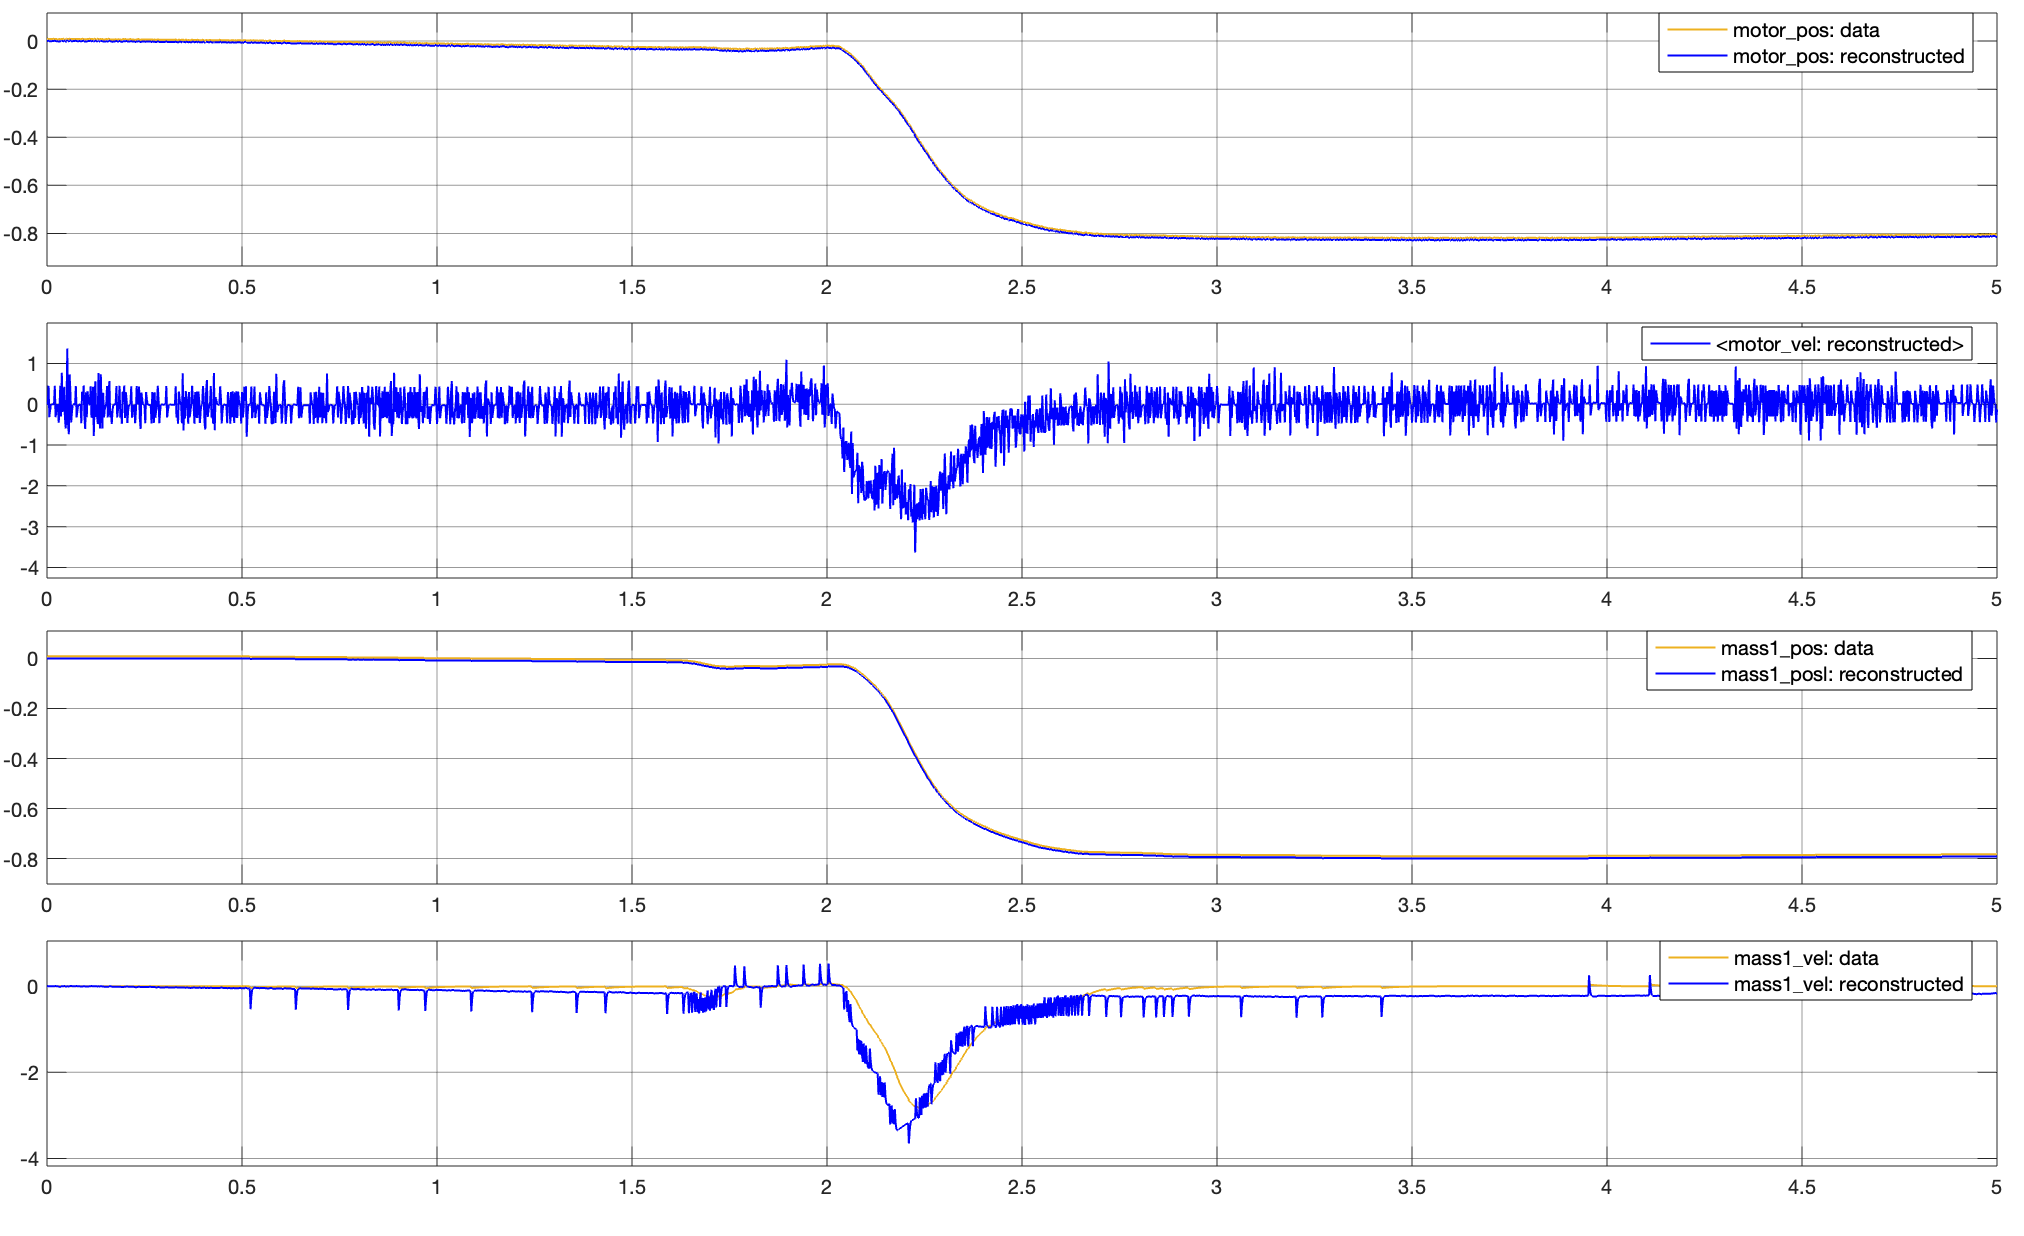
\includegraphics[width=\textwidth]{observer_1dof}
		\subcaption{\acrshort{1-dof} case}
		\label{fig:observer_1dof}
	\end{subfigure}
	\begin{subfigure}{0.45\columnwidth}
		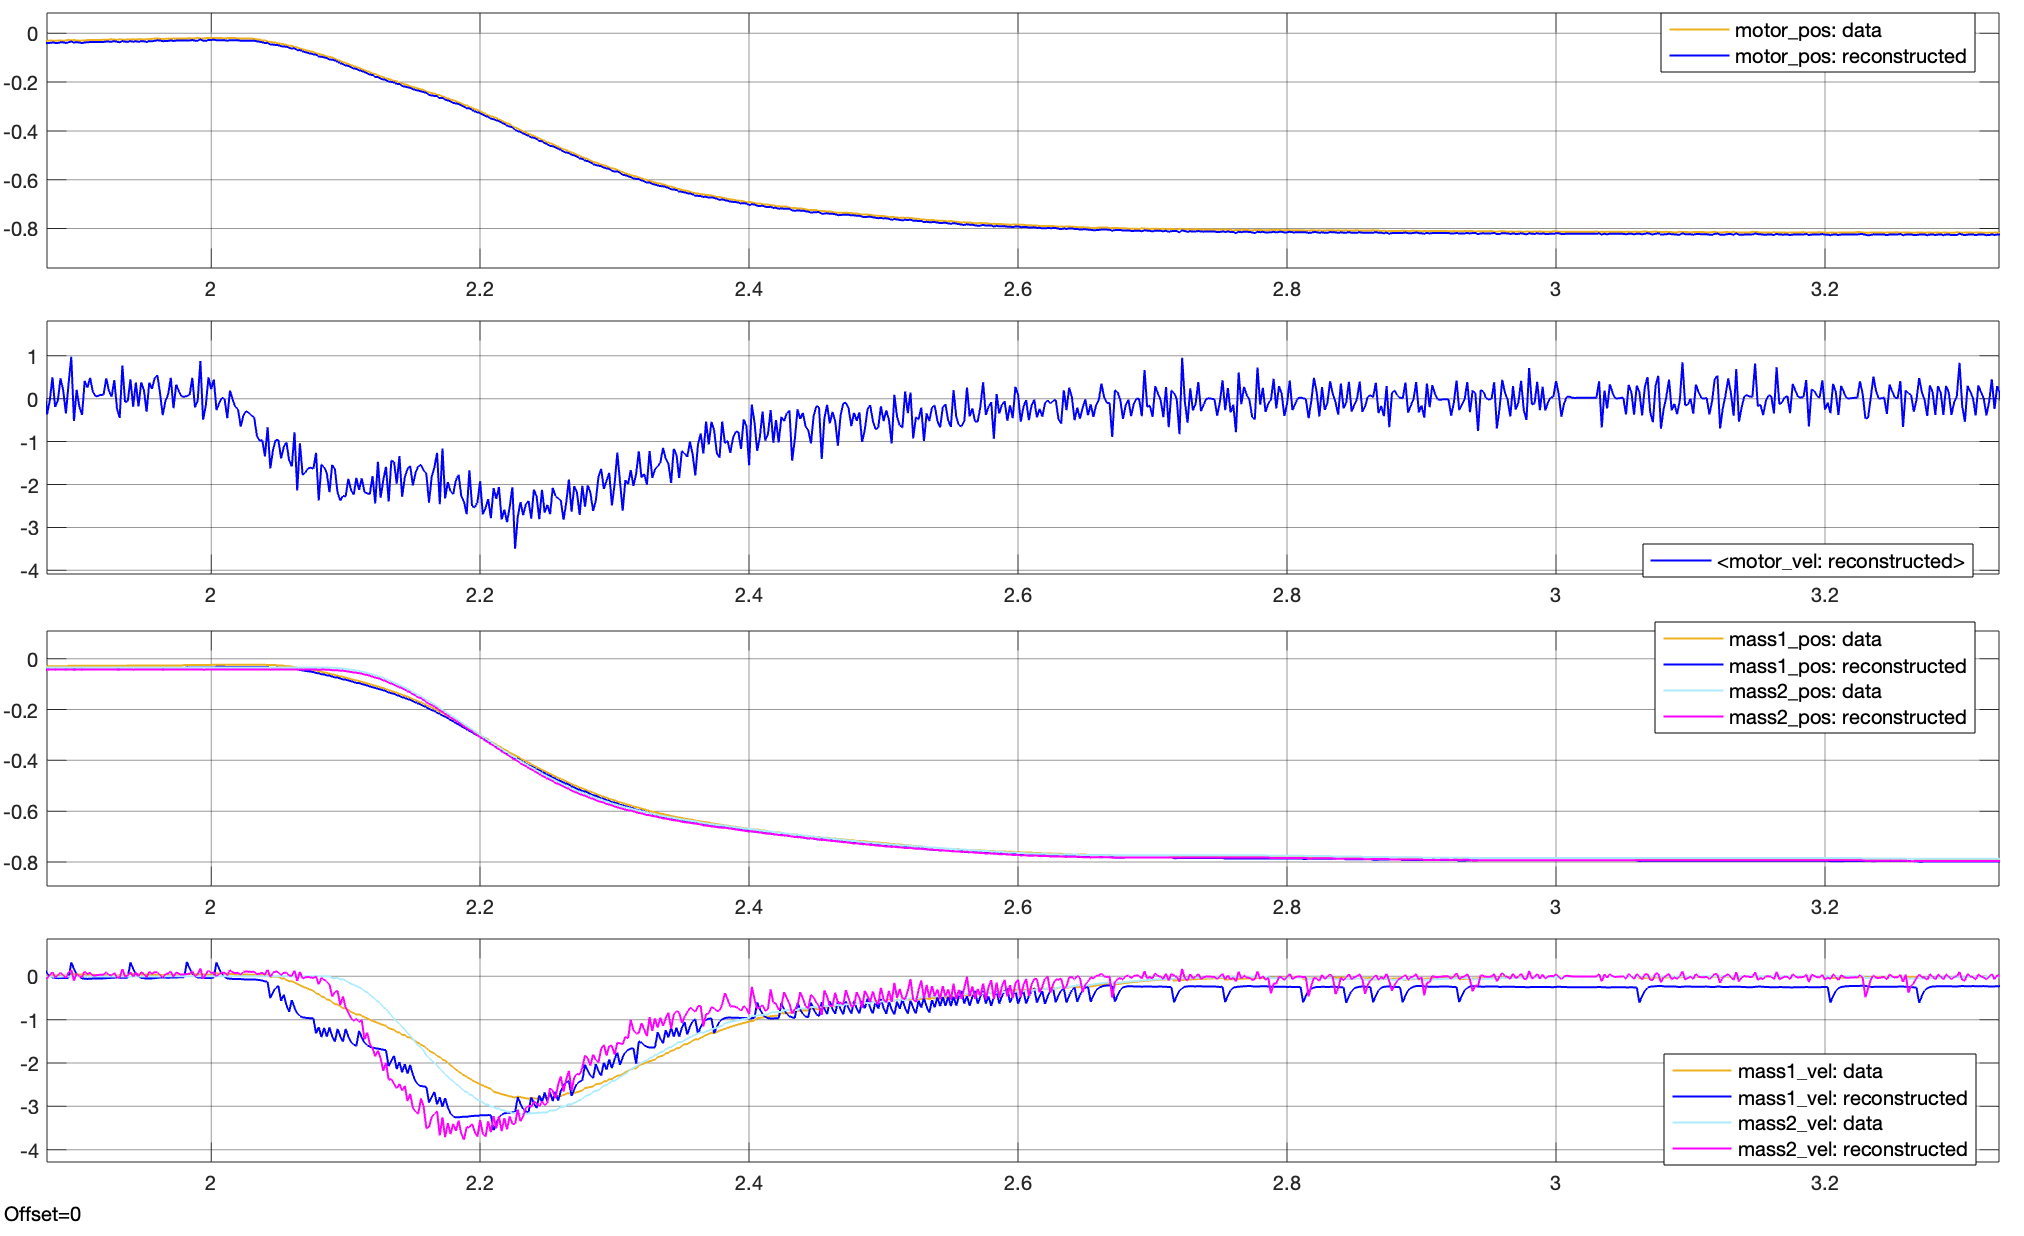
\includegraphics[width=\textwidth]{observer_2dof}
		\subcaption{\acrshort{2-dof} case}
		\label{fig:observer_2dof}
	\end{subfigure}
	\caption{Observer reconstruction compared to available measurements}
\end{figure*}
